\hypertarget{core-scenarios}{\section{Core scenarios}}
\label{sec:core-scenarios}
\FigTop{figures/scenario_structure.pdf}{0.5}{scenario-structure}{\textbf{Scenario structure.} 
Scenarios are what we want the language model to do.
To specify a scenario, we break it down into a \textit{task}, \textit{domain}, and \textit{language}, further subdividing the domain into properties of the text (\textit{what}), speaker (\textit{who}), and the time/circumstances (\textit{when}). 
Examples of scenarios include (question answering, (clinical notes, doctors, now), English) and (toxicity detection, (tweets, Egypt, Internet-era), Arabic).}

We taxonomize scenarios as shown in \reffig{scenario-structure} based on 
(i) a \emph{task} (\eg question answering, summarization), which characterizes what we want a system to do; 
(ii) a \emph{domain} (\eg a Wikipedia 2018 dump), which characterizes the type of data we want the system to do well on;
and
(iii) the \textit{language} or language variety (\eg Spanish).
Tasks, domains, and languages are not atomic or unambiguous constructs: they can be made coarser and finer, but we use them as intuitive \textit{structure} for the space of scenarios.
Given this structure, we deliberately select scenarios based on three overarching principles:
(i) coverage of the space,
(ii) minimality of the set of selected scenarios,
and (iii) prioritizing scenarios that correspond to user-facing tasks.
Alongside feasibility given our resources (which we explicitly acknowledge), this defines the \core scenarios we evaluate on, which we will measure all metrics on. 
In \refsec{missing-scenarios}, we highlight regions of the scenario space that we taxonomize but do not currently cover in our benchmark/scenario selection.

\hypertarget{scenario-taxonomy}{\subsection{Taxonomy}}
\label{sec:generic-scenarios-taxonomy}

\begin{table*}[htp]
\resizebox{\textwidth}{!}{
\begin{tabular}{ll}
\toprule
\textbf{Track} & \textbf{Tasks} \\
\midrule
Computational Social Science and Cultural Analytics & No canonical tasks/not task-centric\\
Dialogue and Interactive Systems & Chit-chat dialogue, task-oriented dialogue \\
Discourse and Pragmatics & Discourse parsing, sentence ordering, coreference resolution\\
Ethics and NLP & Toxicity and hate speech detection, misinformation and fake news detection\\
Generation & Data-to-text generation, \\
Information Extraction & Named entity recognition, entity linking, entity extraction, relation extraction, event extraction, open information extraction \\
Information Retrieval and Text Mining & Information retrieval and passage retrieval\\
Interpretability and Analysis of Models for NLP & No canonical tasks/not task-centric\\
Language Grounding to Vision, Robotics and Beyond & Image captioning, visual question answering, instruction following, navigation \\
Linguistic Theories, Cognitive Modeling, and Psycholinguistics & No canonical tasks/not task-centric\\
Machine Learning for NLP & Language modeling\\
Machine Translation and Multilinguality & Machine translation \\
NLP Applications & No canonical tasks \\
Phonology, Morphology, and Word Segmentation & Tokenization, lemmatization, \\
Question Answering & Question answering and reading comprehension \\
Resources and Evaluation & No canonical tasks/not task-centric\\
Semantics: Lexical & Word sense disambiguation, word sense induction\\
Semantics: Sentence-level Semantics, Textual Inference, and Other Areas & Semantic parsing, natural language inference, semantic role labeling/slot filling, semantic textual similarity, paraphrase detection \\
Sentiment Analysis, Stylistic Analysis, and Argument Mining & Sentiment analysis, style transfer, argument mining, stance detection, opinion mining, text simplification\\
Speech and Multimodality & Text-to-speech, speech-to-text\\
Summarization & Summarization, sentence compression\\
Syntax: Tagging, Chunking and Parsing & POS tagging, chunking, constituency parsing, dependency parsing, grammar induction, grammatical error correction \\
\bottomrule
\end{tabular}}
\caption{\textbf{Taxonomy of tasks.} To taxonomize the space of tasks, we leverage the NLP community’s taxonomy of subareas as codified by the ACL 2022 list of tracks. 
For each track, we then expand it into canonical tasks associated
with that track.}
\label{tab:tasks}
\end{table*}
\paragraph{Tasks.}

Given the ubiquity of natural language, the field of natural language processing (NLP) considers myriad tasks that correspond to language's many functions \citep{jurafsky2000speech}.
It is difficult to derive a space of tasks from first principles, so we compile existing sources of tasks.
Naturally, given NLP is a task-centric field, we begin with tasks that have been extensively studied by the NLP community.
To generate this set, we take the tracks at a major NLP conference (ACL 2022), which reflect the ``relevant topics'' of study in NLP at the time of writing.\footnote{\url{www.2022.aclweb.org/callpapers}}
For each track, we map the associated subarea of NLP to canonical tasks for that track in \reftab{tasks}.
We acknowledge there is some subjectivity in choosing what is ``canonical'', which was only done so as to make this process manageable.

\FigTop{figures/openai_usecase}{0.3}{openai-usecases}{\textbf{Modern use cases for language models.} An assortment of (largely novel/historically unexplored) potential use cases for language models. Figure sourced from \url{https://beta.openai.com/examples/}.}

While these tasks often have long traditions of study in the NLP research community, we make two observations:
(i) these tasks often have important intra-task structure (\eg we refer to all of question answering as one ``task'', whereas the QA community likely would further decompose QA into finer-grained categories \citep{rogers2021qa})
and (ii) while these tasks have (long) traditions of study in NLP research, they are not the only, or even the most societally/economically impactful, tasks.

For example, the deployment of language models as interfaces by OpenAI, Cohere, and AI21 Labs has introduced use cases beyond what the NLP community has historically studied (see \reffig{openai-usecases} and compare to \reftab{tasks}).
In fact, some of these tasks are fundamentally new: the advent of sufficiently capable technology motivates the consideration of tasks that were not previously conceived (or conceived as within scope for algorithmic systems).
Further, these tasks pattern quite differently from what has been traditionally studied in the NLP and AI research communities \citep[see][]{ouyang2022instructions}.
This introduces a fundamental challenge to stating the space of tasks: we will not be able to conceive of the true full space of tasks until we see technology that makes us consider these tasks.
And, more broadly, even articulating (let alone covering) the long tail of known potential use cases remains open. 

\paragraph{Domains.}
Domains are a familiar construct in NLP, yet their imprecision complicates systematic coverage of domains.
We further decompose domains according to 3 W's:
\begin{enumerate}
\item \textbf{What} (genre): the type of text, which captures subject and register differences.
Examples: Wikipedia, social media, news, scientific papers, fiction.
\item \textbf{When} (time period): when the text was created.
Examples: 1980s, pre-Internet, present day (\eg does it cover very recent data?)
\item \textbf{Who} (demographic group): who generated the data or who the data is about.
Examples: Black/White, men/women, children/elderly.
\end{enumerate}
We do not include \textit{where} the text was created (\eg country) and \textit{how} it was created (\eg hand-written, typed, transcribed from speech or sign), but these may also be relevant.
Further, \textit{why} the text was created is closely related to \textit{what} it is.
To be precise, textual data in the input to the language model (\eg the question or the passage, if available, in question answering) and the answer (\eg the summary in summarization) have associated domains that are not necessarily the same.
For simplicity, we will assume a dataset has a single domain corresponding to properties of its inputs, though it would be more precise to consider domains associated with all aspects of the input and output. 

 \begin{figure}[t]
\centering
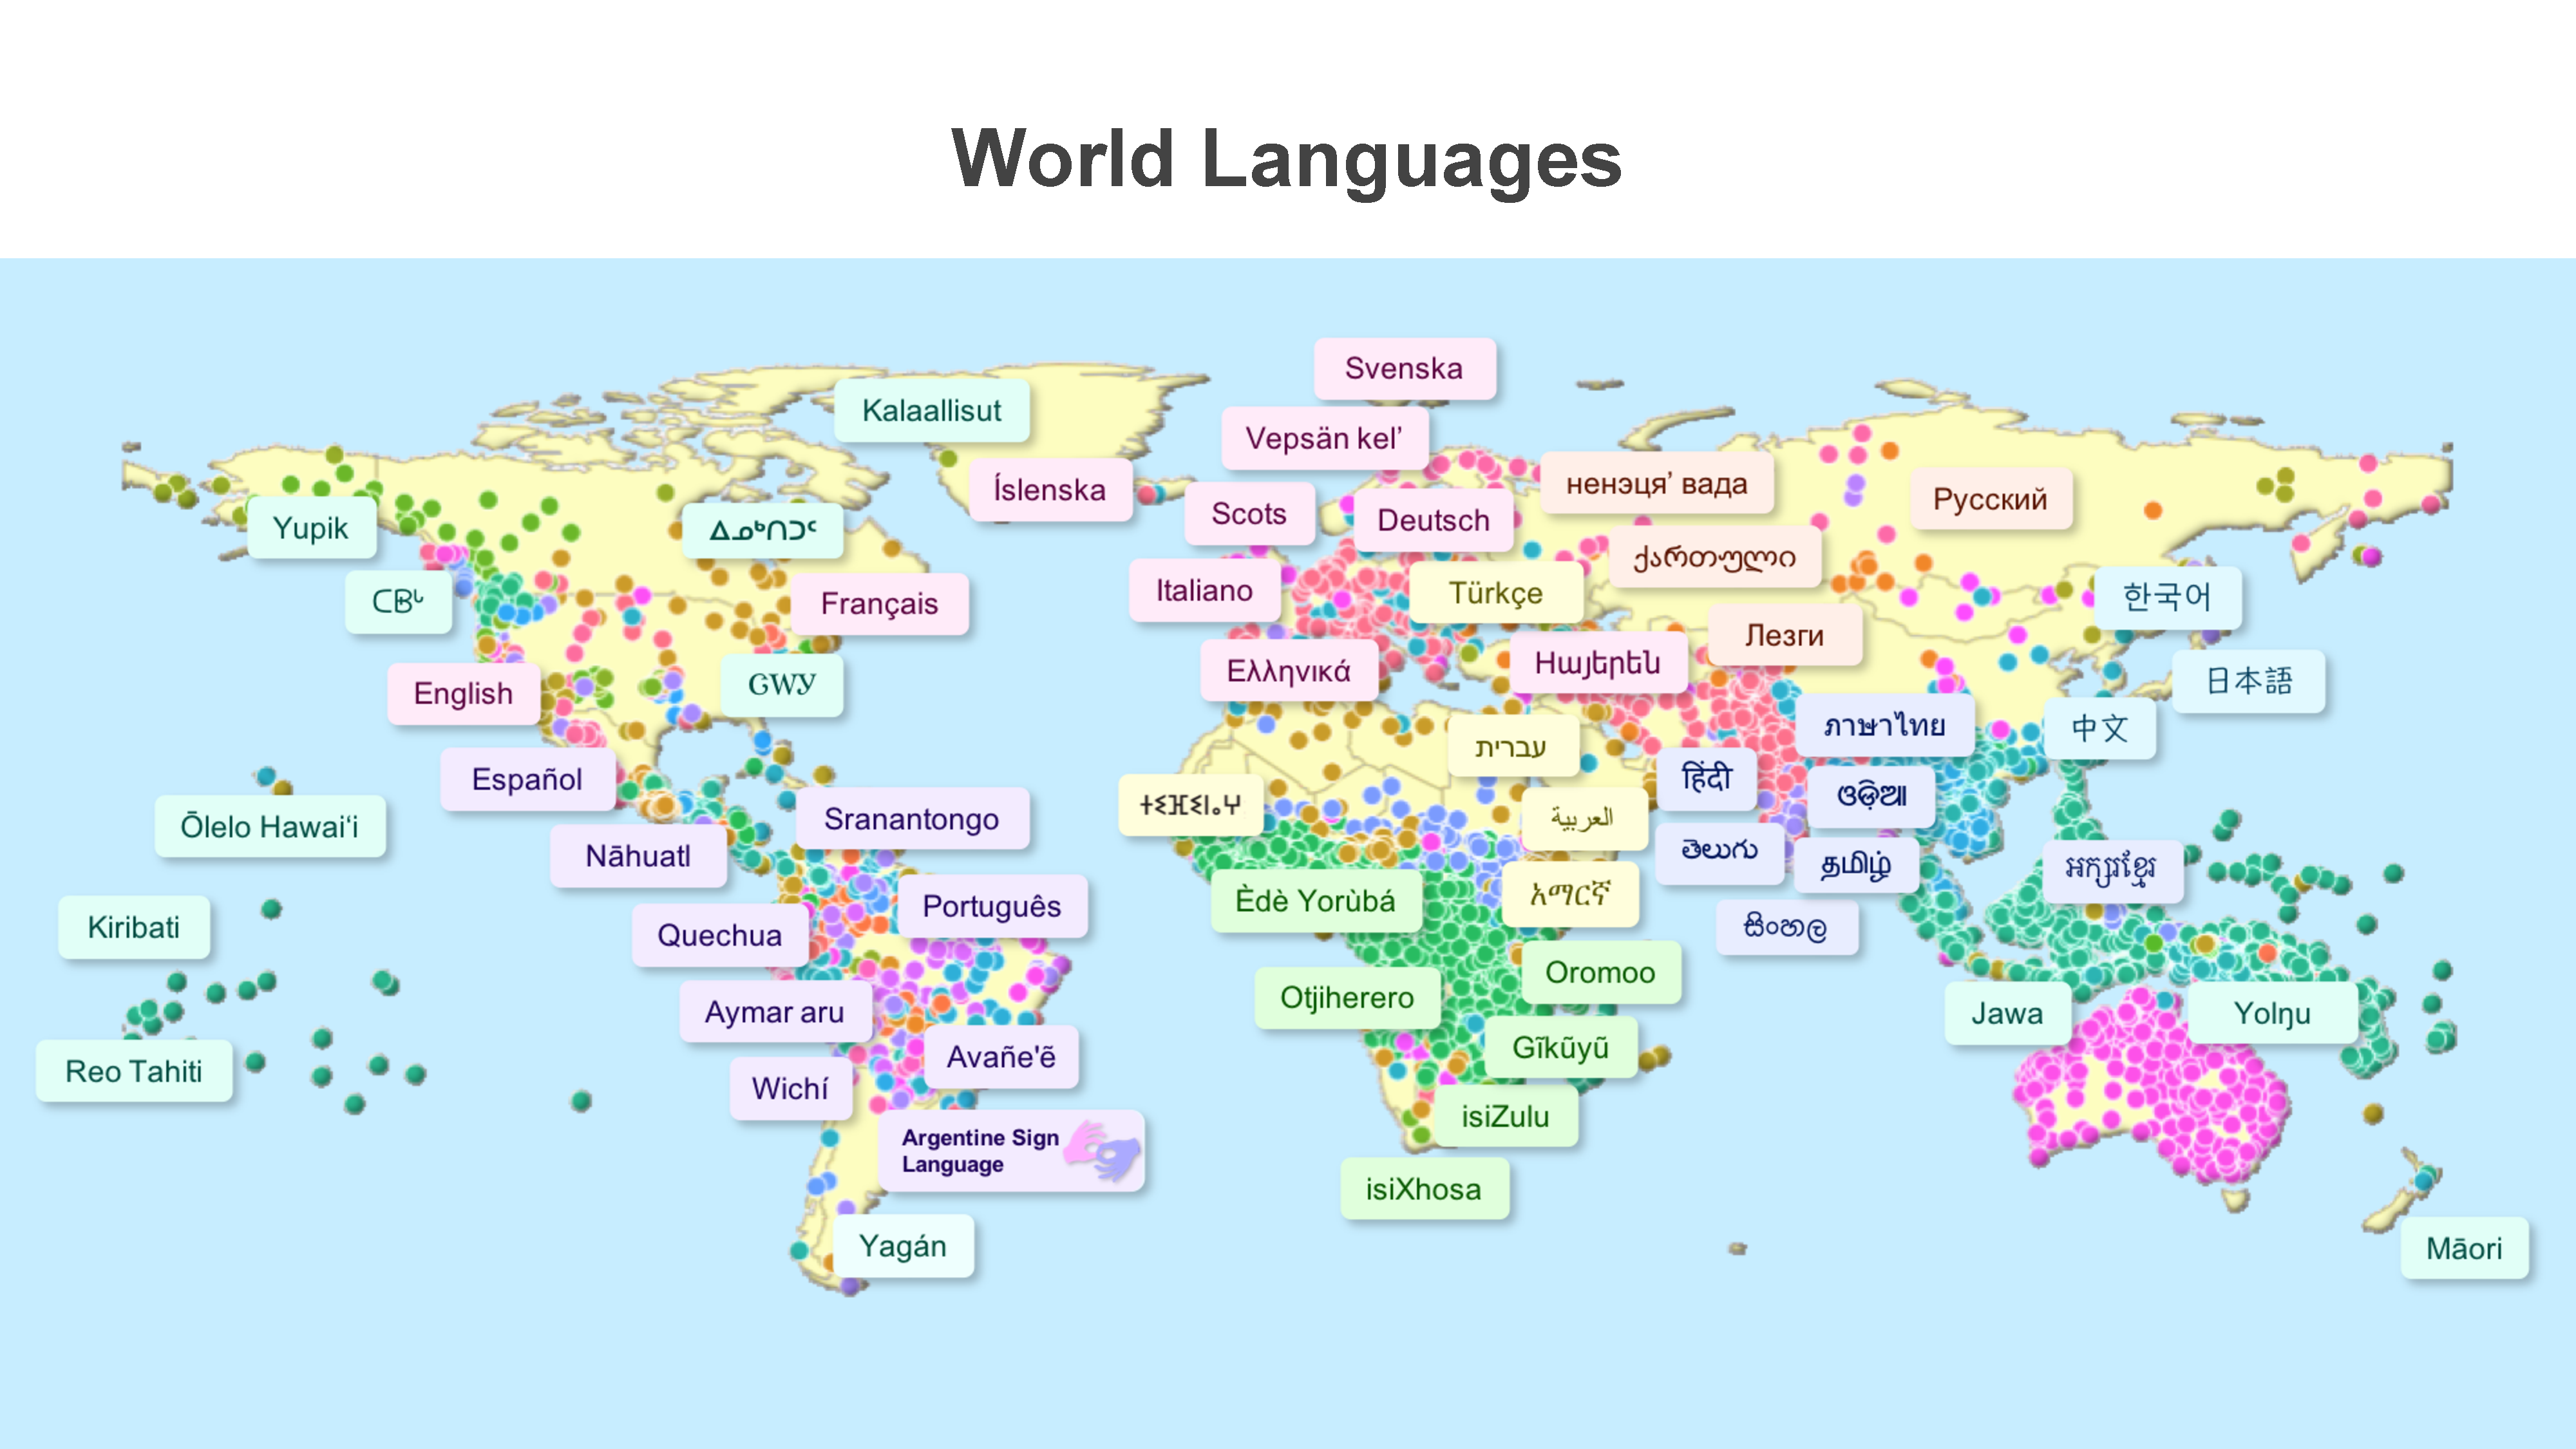
\includegraphics[width=0.9\textwidth]{figures/language_2}
\caption{\label{fig:languages}
\textbf{The world's languages.}
Only a tiny percentage of the world's languages are currently represented in language models. There are over 6,000 languages in the world, with estimates varying due to the inherent uncertainty of what constitutes a separate language \citep{nordhoff2011glottolog}. This map shows the languages of the world, with each dot representing one language and its color indicating the top-level language family. Data is from Glottolog \citep{glottolog}. Figure and caption sourced from \citet[][\S2.1]{bommasani2021opportunities}.}
\end{figure}

\paragraph{Languages.}
The billions of people around the world speak thousands of different languages (see \reffig{languages}).
However, in AI and NLP, the vast majority of work has centered on a few high-resourced languages (\eg English, Chinese), even including languages that have large speaker populations \citep[\eg there are more than 65 million speakers of Fula, a West African language, but few if any NLP resources exist for Fula;][]{nguer2020sencorpus}.
With this in mind, we do not extensively taxonomize the world's languages, as we will focus on predominantly evaluating English-only models (with a few exceptions like \bloom that are clearly multilingual but we evaluate only for English).
Consequently, we instead turn our focus to coverage of English varieties and dialects.
In this regard, we note there are several axes of interest in linguistic typology and sociolinguistics; we point to \citet[][\S2.1]{bommasani2021opportunities} and \citet{joshi2020state} for further discussion. 

\hypertarget{generic-scenarios-selection}{\subsection{Selection}}
\label{sec:generic-scenarios-selection}

As a matter of coverage, ideally, we would evaluate a language model on every scenario (\ie every (task, domain) pair).
However, as we demonstrate in our taxonomy, both tasks and domains themselves are rich and expansive spaces.
For this reason, rather than striving for coverage of scenarios, we instead aim for coverage of tasks, domains, and languages each independently.
This risks not exposing important interactions (\eg we may be especially interested in toxicity detection for text authored by marginalized groups \citep{sap2019risk}), but is a decision we make for practical reasons (\eg availability of datasets, effort to implement scenarios, and computational resources to evaluate LMs on chosen scenarios).

\paragraph{Tasks.}
To select tasks, we begin with the set we described previously.
Since we are studying English language models, we filter infeasible tasks (\eg multimodal tasks or machine translation are not suitable for unimodal English language models).\footnote{We do note that various works have shown these models can achieve nontrivial performance on multimodal tasks (with modalities beyond text) and on other languages (especially as some of these models, most notably \bloom, \glm, and \yalm are trained on sizable datasets in other languages). With that said, we expect that multimodal or multilingual approaches would be more appropriate to achieve reasonable performance for these tasks compared to these models, so we defer such evaluation to future work.}
Of the remaining tasks, we elect to prioritize \textit{user-facing} tasks: we believe these tasks will confer much of the \textit{direct} social impact of language models and aligns with our perspective of language models as \textit{interfaces}. 
Consequently, we filter tasks based on our judgments of what is user-facing.\footnote{We emphasize that this \textit{does not} mean we believe the other tasks are less important nor that they should not be evaluated for in future work.}
This yields the following tasks: 
\textit{question answering}, 
\textit{information retrieval}, 
\textit{summarization}, 
\textit{sentiment analysis}, 
and \textit{toxicity detection}.\footnote{We note that our interpretation of what is user-facing namely excludes tasks that are generally not the subject of applications (\eg natural language inference) as well as many classical NLP tasks that served as intermediaries \citep{jurafsky2000speech} in traditional NLP pipelines (\eg named entity recognition, part-of-speech tagging, syntactic parsing, information extraction). We also do not study interactive tasks such as dialogue, which will be discuss in forthcoming companion work associated with this effort \citep{lee2022interaction}.}
And to provide some coverage of the long tail of tasks, we include \textit{miscellaneous text classification}, which represents the non-standard text classification use cases for language technologies historically and at present for language models. 

\paragraph{Domains and Languages.}
Given that we found it more complicated to arrive at an explicit enumeration of domains compared to tasks,\footnote{Though we note this could be attempted by proposing a taxonomy for each of the 3 W's we consider and then taking the resulting Cartesian product.} we instead focus on domain coverage during our selection of specific datasets to instantiate scenarios.
Similarly, we ensure coverage of the English varieties of different English-speaking countries as well as African American English through targeted evaluations that we discuss in \refsec{language}. 
In doing so, we also demonstrate our desire for a minimal set of evaluations (both because evaluations have costs, so larger sets will be more unwieldy, and producing more results often comes at the cost of clarity on how to sift through them). 
With this in mind, we emphasize that for large regions of the scenario space, specifically in relation to domains (\eg scenarios involving text written by elderly speakers), there exist very few, if any, datasets in NLP.
We hope the community can build on our work by ensuring greater coverage of the domains and scenarios we did not cover in our benchmark by building the necessary and oft-undervalued resources \citep{jo2020archives, paullada2021data, rogers2021changing, jernite2022governance}.
To facilitate this, we explicitly identify specific scenarios that we recommend prioritizing in \refsec{missing-scenarios}. 
We also note that there is more to a dataset than just these axes, which determine how well it operationalizes the desired use case (\eg the quality of crowd-sourced labels in the dataset).  
Having settled on the tasks we will cover and our approach to domain/language coverage, we detail how we selected the particular datasets for each scenario.  

\hypertarget{questionAnswering}{\subsection{Question answering}}
\label{sec:questionAnswering}
Question answering (QA) is a fundamental task in NLP that underpins many real-world applications including web search, chatbots, and personal assistants. 
QA is very broad in terms of the questions that can be asked and the skills that are required to arrive at the answer, covering general language understanding (\refsec{language}), integration of knowledge (\refsec{knowledge}), and reasoning (\refsec{reasoning}) \citep{garder2019qaforamt, rogers2021qa}.
 
\FigTop{figures/scenario_mmlu}{0.5}{question-answering}{\textbf{Example of question answering.} An example instance for question answering from MMLU. Different QA scenarios can have significantly different properties, but this example captures the overall structure of question answering.}

\paragraph{Problem setting.}
In QA, given a question (\eg ``Where was the painter of the Mona Lisa born?''), the task is to predict the correct answer (``Italy'').
The format of question answering may have some variations: in the \textit{open-book} or \textit{reading comprehension} setting, additional context to refer to, such as supporting documents (\eg Wikipedia page of ``Mona Lisa''), is given to the model.
In the \textit{multiple-choice} setting, answer choices to choose from (\eg ``(A) France (B) Italy'') are given to the question.
\reffig{question-answering} depicts an example.

\paragraph{Datasets and selection process.}
There are hundreds of question-answering datasets available in NLP, with a rapid increase in the number of datasets in recent years \citep{rogers2021qa}.
To select question-answering datasets, we prioritized (i) domain coverage, in terms of the domain of the inputs/contexts and (ii) coverage of component skills required for the datasets (\eg we deliberately ensured of datasets that required commonsense knowledge and reasoning). 

We selected the \naturalquestions~\citep{kwiatkowski2019natural},  \narrativeqa~\citep{kovcisky2017narrativeqa}, and \quac~\citep{choi2018quac} datasets to ensure domain coverage as these datasets cover web search queries, stories, and conversational questions (\ie dialogue) respectively.
\naturalquestions~consists of questions from queries to Google search and annotations from Wikipedia; we consider both \textit{open-book} and \textit{closed-book} variants of \naturalquestions.
\narrativeqa~tests reading comprehension through the understanding of books and movie scripts.
\quac~(Question Answering in Context) provides freeform questions and answers which are more open-ended and dependent on context.

To these, we add the \hellaswag~\citep{zellers2019hellaswag}, \openbookqa~\citep{mihaylov2018can}, and \truthfulqa~\citep{stephanielin2021trutfulqa} datasets to ensure coverage of commonsense knowledge and reasoning.
\hellaswag~tests commonsense inference and was created through adversarial filtering to synthesize wrong answers.
\openbookqa~is based on open book exams, with a collection of basic science facts and crowd-sourced multiple-choice questions to test understanding and application of these facts.
\truthfulqa~tests model truthfulness through questions that align with common human misconceptions, spanning law, medicine, finance, and politics, among others, that were adversarially generated using \gptdavinci as the target model.

To further ensure broad coverage of knowledge-intensive question answering across many disciplines, we add the \mmlu~\citep{hendrycks2021measuring} meta-benchmark of 57 constituent datasets. 
\mmlu~(Measuring Massive Multitask Language Understanding) measures multitask accuracy and includes a diverse set of 57 tasks, testing problem solving and general knowledge.

Finally, we add \boolq~\citep{clark2019boolq} which, in addition to \quac, was used to study model robustness to equivariances due to the available contrast set \citep{gardner2020contrast}.
\boolq~is a collection of binary yes/no questions generated through the same process as \naturalquestions.

\hypertarget{informationRetrieval}{\subsection{Information retrieval}}
\label{sec:informationRetrieval}

Information retrieval (IR), which refers to the class of tasks concerned with searching large unstructured collections (often \textit{text} collections), is central to numerous user-facing applications.
IR has a long tradition of study \citep{salton1965smart, salton1971smart,  jones1972statistical, salton1983introduction, manning2008introduction, lin2021pretrained} and is one of the most widely deployed language technologies.
It powers the Web and e-commerce search, and serves as a key component in many knowledge-intensive NLP systems for open-domain question answering or fact checking.

We focus here on the passage ranking task: given a query $q$ and a large corpus $C$ of passages, systems must output a list of the top-$k$ passages from $C$ in decreasing ``relevance'' to $q$. We specifically study this in the context of \textit{re-ranking}: since $C$ is typically extremely large (\eg $|C| > 10M$ passages), we consider only ranking the top-$k$ passages among a set retrieved for $q$ (\ie $M(q)$ where $|M(q)| \ll |C|$) by an efficient external retrieval mechanism \citep[\eg BM25;][]{robertson2009probabilistic}.

IR differs fundamentally from the other tasks we consider in this work, as each test example (\ie a query) entails processing a large set of passages and will likely invoke the LM numerous times to do so.\footnote{Effectively, this means that model outputs come from a very large combinatorial space: they are much more constrained than open-ended generation tasks but much less so than standard classification tasks, setting this scenario apart from many others in terms of its automatic evaluation.} Because of this, IR tasks have received very little attention in the few-shot in-context learning with language models, with the exception of the recent zero-shot approach by \citet{sachan2022improving}.

\FigTop{figures/scenario_msmarco_v3}{0.5}{information-retrieval}{\textbf{Example of information retrieval (passage ranking).} An example instance for information retrieval from MS MARCO.}

\paragraph{Problem setting.}
We address the re-ranking task in a \textit{pointwise} fashion: we formulate the information retrieval problem using prompting as a binary log-probability problem, similar to \citet{nogueira2019passage}: Given a passage $c_i$ and a query $q$, we ask the model whether the passage contains an answer to the query. 
If the model's answer is \texttt{Yes} with a high probability, we rank the corresponding $c_i$ higher, while the \texttt{No} answer with high probability achieves the opposite. 
\reffig{information-retrieval} depicts an example instance.
The rankings produced are then evaluated using standard information retrieval metrics.

\paragraph{Datasets and selection process.} 
We demonstrate the information retrieval task using the MS MARCO ranking datasets. 
While it is originally a question answering task, the retrieval version of MS MARCO is the largest publicly available collection of relevance judgments and has been central to much of the progress in neural IR over the past several years \citep{lin2021pretrained}.

We use the original passage ranking dataset accompanying the public MS MARCO leaderboard\footnote{\url{https://microsoft.github.io/msmarco/}} (\citealt{nguyen2016ms}; henceforth, the \textbf{regular} track) and the dataset from the TREC 2019 Deep Learning track (\citealt{craswell2020overview}; henceforth, the \textbf{TREC} track). Both datasets evaluate retrieval out of a collection of 9M passages from the Web. The regular track contains a large number of queries (e.g., over 500,000 training set queries) with \textit{sparse} relevance judgments: on average, annotators identify only one ``positive'' (relevant) passage for each query, and every other passage is assumed to be a negative. In contrast to this, the TREC track contains only 43 queries that are more rigorously annotated, with over 9,000 query--passage pairs with associated relevance judgments corresponding to the 43 queries.

\hypertarget{summarization}{\subsection{Summarization}}
\label{sec:summarization}
Text summarization is an established research direction in NLP \citep{luhn1958automatic, mani1999advances, sparck1999automatic, nenkova2012survey}, with growing practical importance given the ever-increasing volume of text that would benefit from summarization.
To effectively summarize, systems must identify and yield the core relevant and informative content in the source document while removing less critical information and avoiding redundancy \citep{peyrard2019simple}.
The rise of language models in recent years has dramatically improved summarization capabilities: the ability to generate fluent and coherent human-like text serves as a core primitive towards building better summarization systems \citep{lewis-etal-2020-bart, https://doi.org/10.48550/arxiv.1912.08777}.

\FigTop{figures/scenario_cnn}{0.5}{summarization}{\textbf{Example of summarization.} An example instance for summarization from CNN/DailyMail. Different summarization scenarios can have significantly different properties, but this example captures the overall structure of summarization.}

\paragraph{Problem setting.} 
We formulate text summarization as an unstructured sequence-to-sequence problem, where a document (\eg a CNN news article) is the input and the LM is tasked with generating a summary that resembles the reference summary (\eg the bullet point summary provided by CNN with their article).
\reffig{summarization} provides an example.
This evaluation tests the \textit{abstractive} summarization capabilities of the model, where the model is directly required to generate the summary rather than being explicitly constrained to copying words or larger \textit{extracts} from the input document.

To evaluate model performance, the model-generated summary is compared against a human-authored \textit{reference} summary using automated metrics for overall quality \citep[\texttt{ROUGE-2}; BERTScore;][]{lin-2004-rouge, bert-score}, \textit{faithfulness} \citep{10.1162/tacl_a_00453,fabbri-etal-2022-qafacteval}, and \textit{extractiveness} \citep{grusky2018newsroom}. Faithfulness refers to whether all the information in the model summary is supported by the article \citep{cao2018faithful,durmus-etal-2020-feqa,maynez-etal-2020-faithfulness}. 
Extractiveness refers to the extent to which model summaries involving copying from the input document: the distinction between extractive and abstractive approaches has been widely discussed in the summarization literature \citep[see][]{nenkova2012survey}. 
We compute extractiveness since prior work has shown that current summarization systems tend to be less faithful, on average, whenever they extract less \citep{durmus-etal-2020-feqa,mrini2021rewards,ladhak-etal-2022-faithful}.

We pay special attention to faithfulness as neural models in particular often hallucinate content that diverges from what appears in the document being summarized.
Consequently, it is important to measure and improve the faithfulness of these systems since unfaithful systems may be harmful by potentially spreading misinformation, including dangerous, yet hard to detect  errors, when deployed in real-world settings.
We evaluate the LMs using recently proposed reference-free evaluation metrics that have been shown to get high correlations with human scores for faithfulness \citep{10.1162/tacl_a_00453,fabbri-etal-2022-qafacteval}. 
We note recent work has shown that some reference-free evaluation metrics may be mostly relying on spurious correlations \citep{durmus-etal-2022-spurious}.

% Removed for TMLR
% Given this, we further conducted a human user study to validate and supplement the automated evaluation.

\paragraph{Datasets.} 
There is a growing collection of summarization datasets, including datasets that capture finer-grained and more specific summarization functions (\eg summarizing multiple documents or conditional on a user query).
\citet{bommasani2020intrinsic} show that there is significant diversity in summarization datasets along several axes, which makes selecting a few datasets to represent summarization rather challenging.
Since we are especially interested in model faithfulness in this work (as this is a known failure mode of other neural approaches to summarization), we select the \cnndm~\citep{10.5555/2969239.2969428} and \xsum~\citep{narayan-etal-2018-dont} datasets, which are the most well-studied datasets in the literature on summarization faithfulness.
This also ensures domain coverage of news-type data.
Importantly, these datasets differ along a central axis studied in summarization: \xsum~is a dataset with largely abstractive reference summaries (meaning the string overlap between the document and its summary in the dataset is relatively small on average), whereas \cnndm~is a dataset with largely extractive reference summaries. 
However, these datasets do not suffice in representing the full diversity of summarization, and we encourage future work to expand on our benchmark along this axis (\eg add datasets from domains beyond news), particularly towards domains where there is greater demand for summaries \citep[see][]{reiter2022summarization}.
And we especially highlight that these two datasets have been the subject of critique, and that broader change is required for dataset and evaluation design in summarization and natural language generation \citep{gehrmann2022repairing, reiter2022summarization}. 

\hypertarget{sentimentanalysis}{\subsection{Sentiment analysis}}
\label{sec:sentimentanalysis}

Sentiment analysis is an iconic task in NLP \citep[see][\S4]{jurafsky2000speech} that has led to widespread deployment in finance, health, social media, with applications in many sectors in relation to customer reviews of products and services \citep{pang2008opinion}.
Since its popularization by \citet{turney2002thumbs} and \citet{pang2002thumbs}, sentiment analysis has blossomed into its own subarea in the field with many works broadening and deepening the study of sentiment from its initial binary text-classification framing \citep{wiebe2005annotating, mcauley2012learning, socher2013recursive, nakov2016semeval, potts2021dynasent}.

\FigTop{figures/scenario_imdb}{0.5}{sentiment-analysis}{\textbf{Example of sentiment analysis.} An example instance for sentiment analysis from \imdb.}

\paragraph{Problem setting.}
Given an input sequence (\eg ``Caddyshack II does NO justice for the caddysack. thin plot \dots movie should have been destroyed when the script was written.''), the goal of sentiment analysis is to predict the sentiment label (``Negative''). 
\reffig{sentiment-analysis} provides an example.

\paragraph{Datasets and selection process.}
Numerous datasets have been put forth for sentiment analysis, including increasingly fine-grained and complex datasets in recent years \citep[cf.][]{potts2021dynasent}.
Of these, only for practical reasons due to engineering resources to implement scenarios, we elected to only include one sentiment analysis dataset.
Of the available sentiment analysis datasets, we selected the \imdb~dataset \citep{maas2011imdb}, as it had the unique resource of a contrast set \citep{gardner2020contrast}, which enables the measurement of robustness to equivariances (which we found difficult to measure otherwise).
\imdb~is constructed from IMDB movie reviews, where users rate movies from 1--10.
These ratings are discretized to a binary space, with reviews with a score at most 4 being labeled negative and reviews with a score at least 7 being labeled positive. 
As discussed in \citet{potts2021dynasent}, we emphasize that sentiment analysis is more diverse and can be more complex: we encourage future work to expand on our benchmark along this axis (\eg add datasets from domains where sentiment analysis is actively deployed).

\hypertarget{toxicity-detection}{\subsection{Toxicity detection}}
\label{sec:toxicity-detection}

Toxicity detection (and the related tasks of hate speech and abusive language detection) is the task of identifying when input data contains toxic content, which originated due to the need for content moderation on the Internet \citep{schmidt2017survey, rauh2022characteristics}.
Automated detection of toxic content has become increasingly critical to content moderation policies at major companies and social media platforms such as Meta, Twitter, and Reddit, including recent deployments that center language models.\footnote{\url{https://ai.facebook.com/blog/how-facebook-uses-super-efficient-ai-models-to-detect-hate-speech/}}
However, both the task's framing and the deployment of automated systems for the task has been the subject of intense debate: critiques of the task have noted that 
(i) the study of toxicity is overly reductive and divorced from use cases \citep{diaz2022accounting}, 
(ii) standard datasets often lack sufficient context to make reliable judgments \citep{pavlopoulos2020toxicity, hovy2021importance},  
and (iii) the construct of toxicity depends on the annotator \citep{sap2019risk, gordon2022jury}.
Ultimately, specific definitions of toxicity can be sensitive to social group membership as well as notions of social status and privilege, such that their interpretation causes disproportionate impact to  members of marginalized groups \citep{welbl2021challenges}.

We emphasize that the stakes for toxicity detection are as high as they can be. Failures in content moderation due to failures in toxicity detection have contributed to serious human rights violations \citep[such as the Rohingya genocide in Myanmar;][]{stecklow2018report,BSR2018HRIA,OHCHR2018report} and have put democracies around the world under stress \citep{persily_tucker_2020}. Some of these failures have been attributed to an absence of human moderators with sufficient linguistic and cultural competence in the countries and communities where risks of ethnic conflict arise. Given language models’ subpar performance in languages that are not dominant in the field of machine learning, there is a legitimate concern that automated moderation could exacerbate the problem. 

\FigTop{figures/scenario_civilcomments}{0.5}{toxicity-detection}{\textbf{Example of toxicity detection.} An example instance for toxicity detection from \civilcomments.}

\paragraph{Problem setting.}
Akin to sentiment analysis, for toxicity detection we consider the binary classification problem of determining whether the input sequence (\eg ``Russ Newell please show me where the K12 education has been `gutted'. Simply preposterous.'') is or is not toxic.
We directly ask the model to determine if the text is toxic by prompting with ``Question: Is the passage above toxic?'', where we use the term ``toxic'' to match the classification category used to label the data.
An example is provided in \reffig{toxicity-detection}.

\paragraph{Datasets and selection process.} 
In recent years, a growing collection of toxicity detection datasets has emerged.
Of these, we choose the \civilcomments~dataset \citep{borkan2019nuanced} from the WILDS benchmark \citep{koh2021wilds}.
Specifically, when compared with other comparable toxicity detection datasets, the dataset includes metadata annotations on the data subjects that are mentioned in the text (and, therefore, the recipients of toxicity).
This allows us to measure performance disparities with respect to several demographic groups and categories that was otherwise difficult, which is especially important given the subjective nature of toxicity \citep{sap2019risk, gordon2022jury}.
\civilcomments~uses comments from the Civil Comments platform from 2015--2017, with comments drawn from 50 English-language news sites across the world.

\hypertarget{textclassification}{\subsection{Miscellaneous text classification}}
\label{sec:textclassification}
Text classification and categorization refers to the family of NLP tasks where an input sequence (\eg sentence, document) is assigned a label.
Text classification has a long history in NLP \citep[see][]{yang1997comparative, yang1999evaluation, joachims1998svm, aggarwal2012survey} with tasks such as language identification, sentiment analysis, topic classification, and toxicity detection being some of the most prominent tasks within this family.
However, beyond these prominent tasks, there is a long and growing tail of miscellaneous text classification tasks with use cases throughout society.\footnote{See \url{https://openai.com/blog/gpt-3-apps/}.}
While not all of these tasks have established traditions and literatures in academia, we expect these tasks comprise an important class of evaluations for assessing the practical utility of language models. 

\FigTop{figures/scenario_raft}{0.5}{misc-text-classification}{\textbf{Example of miscellaneous text classification.} An example instance for miscellaneous text classification from \raft (subset=Banking77).}

\paragraph{Problem setting.}
Akin to sentiment analysis, the input will be a text sequence (\eg ``Query: I withdrew cash and I think the exchange rate is wrong.'') and the output will be a categorical label (``wrong exchange rate for cash withdrawal'') that the model is expected to directly predict.  
Unlike sentiment analysis and toxicity detection, since the tasks do not necessarily correspond to a term and may be more complex (\eg classify banking customer service queries), we provide further instructions that designate the task (\eg identify the text is a banking customer service query and the model should classify it into one of the 77 provided categories). 
An example is provided in \reffig{misc-text-classification}.

\paragraph{Datasets and selection process.} 
Unlike other tasks, essentially by construction, it is near-impossible to enumerate, let alone represent, all the non-standard text classification tasks that are useful.
For this reason, we turn to \raft~\citep{alex2021raft}, which is a collection of 11 ecologically-valid tasks with real applications: adverse drug effect detection (ADE), banking customer service query classification (Banking77), harmful applications detection in NeurIPS impact statements (NeurIPS), classification of level of adult English (OneStopEnglish), detection of overruling in legal statements (Overruling), institution classification of semiconductor organizations (Semiconductor), classification of papers that advance past screening for charitable donations (SystematicReview), classification of transformative artificial intelligence research (TAI), detection of unfair terms of service (ToS), hate speech detection of Tweets (TweetEvalHate), and complaint detection in Tweets (TweetComplaints). 
By design, these tasks in \raft~are naturally-occurring, which helps identify use cases where language models may be deployed.
Since the labels for the full test set are private, we hold out a subset of the public training set for evaluation.